\RequirePackage{luatex85}
\documentclass[tikz]{standalone}
% Default preamble
\usepackage{pgfplots}
\pgfplotsset{compat=newest}
\usepgfplotslibrary{groupplots}
\usepgfplotslibrary{polar}
\usepgfplotslibrary{smithchart}
\usepgfplotslibrary{statistics}
\usepgfplotslibrary{dateplot}
\usepgfplotslibrary{ternary}
% Custom preamble from global variable:
\usetikzlibrary{patterns}
\usepackage{xcolor}
\definecolor{cred}{HTML}{ED1C24}
\definecolor{cgrey}{HTML}{7F7F7F}
\definecolor{cblue}{HTML}{00A2E8}
\definecolor{cgreen}{HTML}{22B14C}
\definecolor{cyellow}{HTML}{FFF200}
\definecolor{corange}{HTML}{EA7904}
\definecolor{cpurple}{HTML}{9100FC}
\definecolor{julia1}{HTML}{1F77B4}
\definecolor{julia2}{HTML}{FF7F0E}
\definecolor{julia3}{HTML}{2CA02C}
\definecolor{julia4}{HTML}{D62728}
\begin{document}
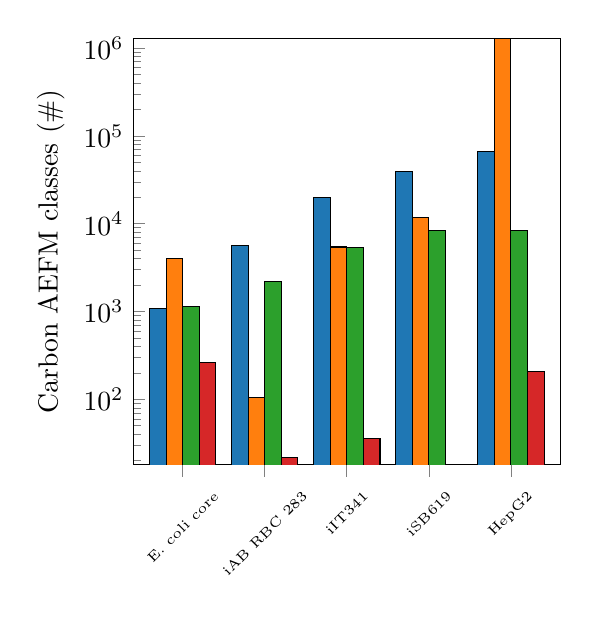
\begin{tikzpicture}
\begin{semilogyaxis}[height={7cm}, width={7cm}, ybar = 0pt, xmajorgrids={false}, ymajorgrids={false}, xtick pos = bottom, ytick pos = left, bar width = 6pt, enlarge x limits = 0.15, enlarge y limits = false, legend image code/.code={\draw [#1] (0cm,-0.1cm) rectangle (0.2cm,0.25cm); }, legend style={legend columns={2}, font=\tiny}, xmax={5}, xtick={1,2,3,4,5}, xticklabels={E. coli core,iAB RBC 283,iIT341,iSB619,HepG2}, xticklabel style = {font=\tiny, align=center,rotate=45}, ylabel={Carbon AEFM classes (\#)}, ymin={0}]
    \addplot[black, fill=julia1]
        coordinates {
            (1,1095)
            (2,5630)
            (3,19795)
            (4,39332)
            (5,66376)
        }
        ;
    \addplot[black, fill=julia2]
        coordinates {
            (1,4014)
            (2,106)
            (3,5432)
            (4,11696)
            (5,1302980)
        }
        ;
    \addplot[black, fill=julia3]
        coordinates {
            (1,1149)
            (2,2200)
            (3,5370)
            (4,8398)
            (5,8375)
        }
        ;
    \addplot[black, fill=julia4]
        coordinates {
            (1,261)
            (2,22)
            (3,36)
            (4,18)
            (5,206)
        }
        ;
\end{semilogyaxis}
\end{tikzpicture}
\end{document}
